\documentclass{article}

% set font encoding for PDFLaTeX, XeLaTeX, or LuaTeX
\usepackage{ifxetex,ifluatex}
\if\ifxetex T\else\ifluatex T\else F\fi\fi T%
  \usepackage{fontspec}
\else
  \usepackage[T1]{fontenc}
  \usepackage[italian]{babel}
  \usepackage[utf8]{inputenc}
  \usepackage{lmodern}
\fi

\usepackage{hyperref}
\usepackage[table]{xcolor}
\usepackage{booktabs}
\usepackage{float}
\usepackage[pdftex]{graphicx}
\usepackage[a4paper, total={6in, 8in}]{geometry}
\usepackage{caption} 
\captionsetup[table]{position=bottom} 

\title{Documentazione progetto "Smart calendar for business"}
\author{Filippo Lazzari [matricola], Mauro Riva [1053644] e Marco Rodolfi [1040347]}
\date{}

\usepackage{sagetex}
\usepackage{pythontex}

\begin{document}
\maketitle
\section{Iterazione 0}
\subsection{Introduzione e utilizzo del sistema}
L'obiettivo di questo progetto è quello di poter organizzare i turni di un'azienda, specialmente per quelli che devono gestire turni a rotazione che devono essere sempre presenti per il servizio clienti, come tutti i servizi di ristorazione, per esempio. 

Questo è stato idealizzato come tre componenti distinte all'interno dell'applicativo:
\begin{enumerate}
\item Una parte lato server che gestirà i client tramite chiamate REST e farà girare l'algoritmo per ottimizzare la selezione dei turni.
\item Una parte web che gestisca la registrazione dell'azienda al servizio.
\item Un'applicativo per dispositivi Android che permetta agli utenti dell'azienda di gestire il proprio stato e richiedere malattie/straordinari.
\end{enumerate}
\subsubsection{Il server dell'applicativo}
Questo deve poter gestire più di una singola azienda e verrà gestito direttamente da chi gestisce il servizio. Lo stesso quindi deve poter permettere la registrazione di più aziende sullo stesso sistema. Per permettere di gestire le decisioni dell'algoritmo, è richiesta un'interfaccia web che permetta la gestione da parte della stessa azienda.
\subsubsection{L'applicativo Android}
Per permettere una maggiore flessibilità di gestione da parte dei dipendenti che lavorano, abbiamo pensato di creare un'applicativo Android che permetta di gestire il proprio stato all'interno dell'azienda, richiedere malattie e verificare i propri straordinari. La comunicazione verso il server è quindi gestita tramite chiamate REST.
\subsubsection{L'algoritmo}
L'algoritmo deve saper gestire dinamicamente l'allocazione dei turni e poter gestire i turni scoperti verificando se persone di altre sedi della stessa azienda e che coprano ruoli identici possano sostituire le persone nella stessa, tenendo conto sia dell'eventuale distanza dalla sede in cui dovrebbero coprire il turno sia delle loro ore massime di straordinari imposti per limiti di legge.
\subsection{Requisiti funzionali e casi d'uso}
I casi d'uso pensati per il nostro software sono disegnati qua sotto:
\begin{figure}[H]
  \centering
  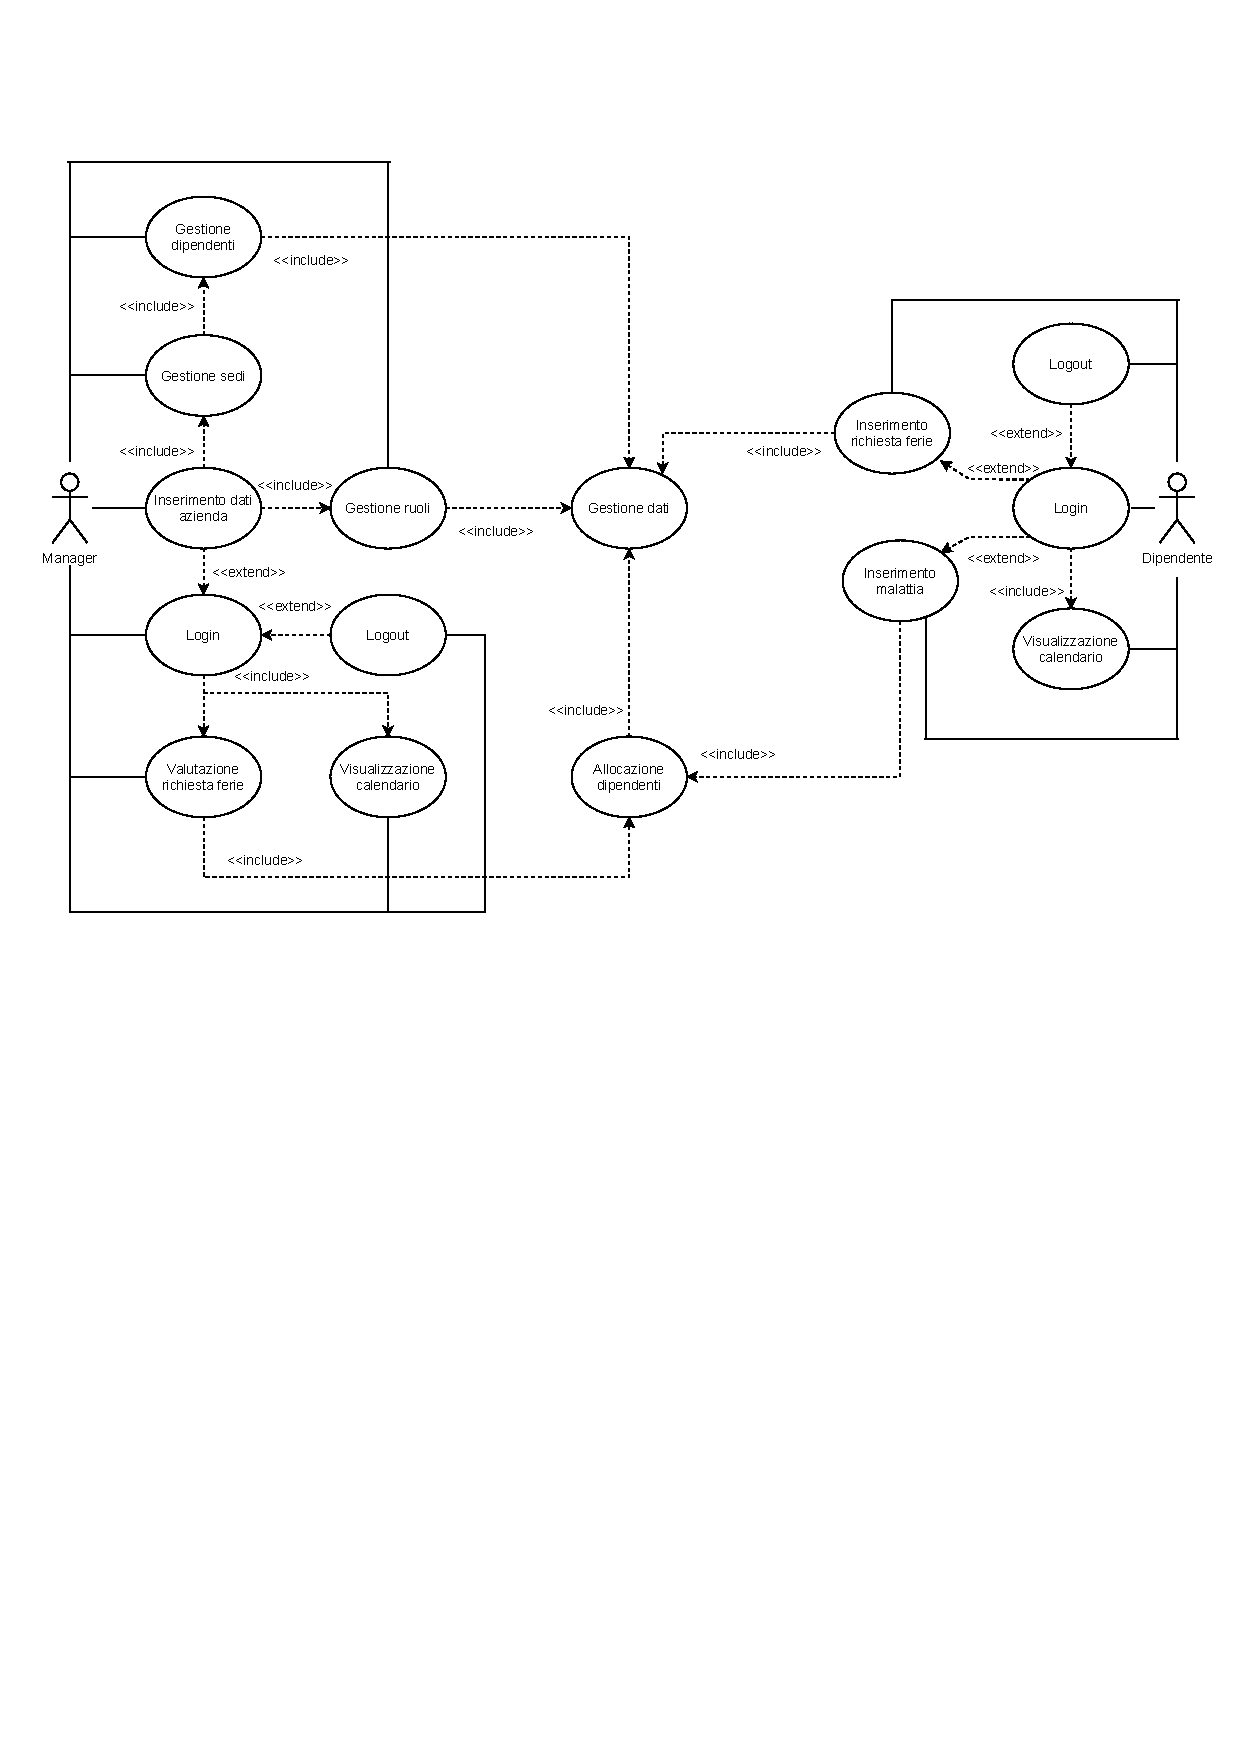
\includegraphics[angle=90,origin=c,width=\paperwidth]{UseCase.pdf}
  \caption{Casi d'uso pensati}
\end{figure}
Questa prima tabella rappresenta i casi d'uso iniziali che abbiamo ritenuto importanti da includere già all'inizio del nostro progetto:
\def\arraystretch{1.5}%  1 is the default, change whatever you need
\begin{table}[H]
\centering
\begin{tabular}[t]{cc}
\toprule
\textsc{Identificativo} & \textsc{Nome Funzione}\\\midrule
UC1 & Inserimento dati azienda \\
UC2 & Login \\
UC3 & Logout \\
UC4 & Gestione ruoli \\
UC5 & Gestione sedi \\
UC6 & Gestione dipendenti \\
UC7 & Algoritmo di organizzazione dei dipendenti\\\bottomrule
\end{tabular}
\caption{\label{tab:high-priority}Alta priorità}
\end{table}
Questa seconda tabella invece stava ad indicare cosa ci sarebbe piaciuto includere come idea ma non necessarie per le prima iterazione:
\begin{table}[H]
\centering
\begin{tabular}[t]{cc}
\toprule
\textsc{Identificativo} & \textsc{Nome Funzione}\\\midrule
UC8 & Visualizzazione calendario \\
UC9 & Login dipendenti \\
UC10 & Inserimento malattia \\
UC11 & Inserimento richiesta di ferie \\
UC12 & Valutazione richiesta di ferie \\\bottomrule
\end{tabular}
\caption{\label{tab:med-priority}Media priorità}
\end{table}
Infine queste sono casi d'uso interessanti da avere come aggiunta ma non necessariamente essenziali per l'applicativo stesso:
\begin{table}[H]
\centering
\begin{tabular}[t]{cc}
\toprule
\textsc{Identificativo} & \textsc{Nome Funzione}\\\midrule
UC13 & Personalizzazione calendario\\
UC14 & Visual. avanzata della situazione dei dip. \\
UC15 & Limitazioni nell'inserimento delle ferie\\
UC16 & Modifica credenziali di accesso \\\bottomrule
\end{tabular}
\caption{\label{tab:low-priority}Bassa priorità}
\end{table}
\subsection{Requisiti non funzionali}
\subsubsection{Usabilità}
L'usabilità é stata considerata nella creazione dell'applicativo Android, permettendo una più facile gestione dei turni da parte degli utenti dell'azienda.
\subsubsection{Manutenibilità}
\subsubsection{Efficienza}
Algoritmo? Che altro?
\subsection{Design Pattern}
\subsection{Toolchain utilizzati}
\begin{table}[H]
\centering
\begin{tabular}[t]{ll}
\toprule
\textsc{Nome Toolchain} & \textsc{Utilizzo}\\\midrule
IntelliJ IDEA Ultimate & Utilizzato come IDE di sviluppo per backend\\
Android Studio & Utilizzato per lo sviluppo dell'applicativo Android\\
Git \& Gitlab & Software e piattaforma per gestire la distribuzione del codice sorgente\\
Cocalc & Piattaforma utilizzata per la scrittura collaborativa della documentazione \LaTeX\\
Java 17 & Linguaggio di programmazione usato per il server e l'applicativo Android \\
Draw.io & Piattaforma utilizzata per creare diagrammi UML\\
Spring Boot & Il framework utilizzato lato server per il suo funzionamento\\
Spring Data JPA & Interfaccia per l'astrazione della base di dati\\
JGraphT & Libreria per i grafi utilizzata per lo sviluppo dell'algoritmo\\
PostgreSQL & Il DB scelto per gestire la base di dati stessa \\\bottomrule
\end{tabular}
\caption{\label{tab:toolchain}Toolchain Utilizzati}
\end{table}

\end{document}

